\section{Infrastruttura IT}
\subsection{Descrizione}
\subsection{Apparati Utilizzati}
\subsubsection{Descrizione}
\subsubsection{Data server}
\subsubsection{Application server}
\subsubsection{API server}
\subsubsection{Web server}
\subsection{Progetto di rete} 
Ho progettato la rete per la sede centrale dell'azienda usando Cisco Packet Tracer 8.0, nelle etichette da me inserite sono riportati gli indirizzi IP degni di nota e le informazioni relative alle 4 sottoreti create. Il file è stato caricato insieme a tutto il progetto nell'apposita repository creata su GitHub e \href{https://github.com/MauroPello/elaborato}{raggiungibile qui} \cite{GitHub}. 
\begin{sidewaysfigure}
    \centering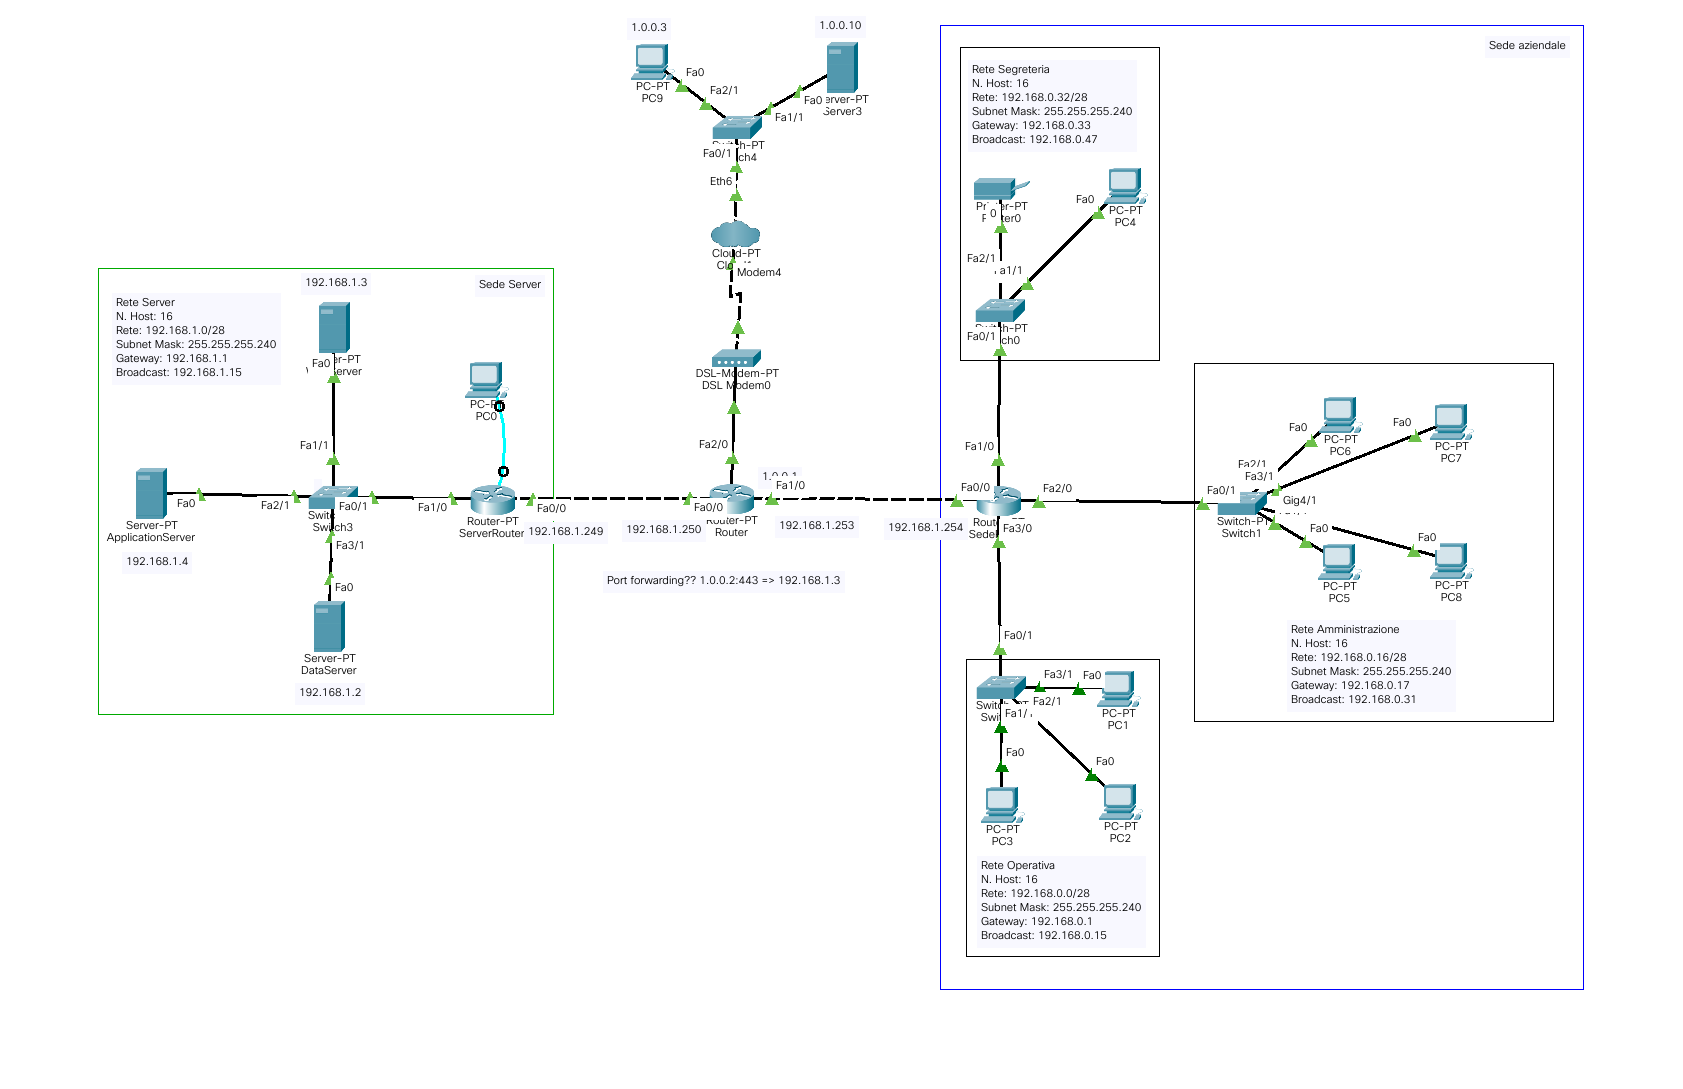
\includegraphics[scale=.48]{images/rete.png}
    \caption{Progetto della rete scritto con Cisco Packet Tracer. }
\end{sidewaysfigure}
\clearpage